% ------------------------------------
% INTRODUCTION
% ------------------------------------
\section{Introduction}
\label{sec:introduction}
In recent years computing is becoming more ubiquitous in the physical world. This notion of ubicomp was introduced by Weiser \cite{weiser1999origins}, where the concept of
smart environment was defined as ``\textit{a physical world richly and invisibly interwoven with sensors, actuators, displays, and computational elements, embedded seamlessly in the everyday
objects of our lives and connected through a continuous network}''. Through the years, technology advances such as the creation of the Internet contributes to achieving the ubicomp's vision
which enables individual devices to communicate between themselves from any part of the world \cite{gubbi2013internet}. In Weiser's vision of ubiquitous computing, information seamlessly moves
in and out of attention as automation gives way to human interaction \cite{weiser1991computer}.\\

The progress towards ubiquitous computing has been slower than expected \cite{greenfield2010everyware}, another approaches for ubiquitous computing that constrasts with Weiser vision becomes relevant.
Rogers' proposes an approach which focuses in designing technologies for engaging user experiences that in a creative and constructive way, extend the peoples' capabilities \cite{rogers2006moving}.
Rogers points that ubiquitous technologies can be developed not only for individuals, but for particular domains that can be set up and customized by an organization according its needs, such as
agriculture, retailing and logistics.\\

Actually, Weiser vision is close to becoming reality thanks to the Internet of Things and Cloud Computing \cite{caceres2012ubicomp}. This world where things are connected through a continuous network
is a vision thats represents the Internet of Things (IoT). In this vision, physical items are continuously connected to the virtual world and can act as remotely physical access points to Internet Services.
The Internet of Things would make computing truly ubiquitous \cite{mattern2010internet}.\\

A common scenario where the Internet of Things paradigm is applied are smart environments \cite{atzori2010internet}, which in this document are designated as smart places.
In the context of this work, a smart place can be defined as an ecosystem composed by smart objects such as RFID tags and sensors, that are able to acquire knowledge about this environment and also to
adapt this inhabitants in order to improve their experience in that environment \cite{cook2004smart}.
In particular, the deployment of IoT applications in a smart place is a challenge today due the heterogeneity of the smart objects that are present in a smart place
and also because the required infrastructure. In order to decrease the complexity of the deployment of an IoT application in a smart place, the Cloud computing paradigm allows the
virtualization of the required physical infrastructure. Nowadays the server infrastructure needed by IoT applications can be virtualized by Cloud providers, which gives more flexibility and reduces
the costs in the deployment of an IoT application.
Therefore, another challenge concerns the heterogeneity of a smart place, more precisely the variety of smart objects that can be inside of a given place. Many of these objects uses different communication
protocols and drivers to communicate with devices, thus the configuration of this objects must be manually handled, which makes the integration of these objects in the deployment of IoT applications in a smart place
an inefficient process.\\
% -------------------------------------
% INTERNET OF THINGS
% -------------------------------------
\subsection{Internet of Things}
\label{sub:internet_of_things}
The Internet of Things is a concept in which the virtual world of information technology integrates seamlessly
with the real world of physical things \cite{Uckelmann:2011:AIT:2018904}. Through the amount of computer and network devices
available nowadays, the real world becomes accessible to business and everyday scenarios.\\

A more precise definition of what does the Internet of Things was formulated in the Strategic Research Agenda of the Cluster of European Research Projects
on the Internet of Things (CERP-IoT 2009):\\

``\textit{In the IoT, `things' are expected to become active participants in business, information and social
processes where they are enabled (...) by exchanging data and information  sensed about the environment, while reacting autonomously to the `real/physical world'
events and influencing it by running processes that trigger actions and create services with or without direct human intervention. Interfaces in the form of services
facilitate interactions with these `smart things' over the Internet (...) taking into account security and privacy issues.}''\\

IoT provides access to a more detailed information, which results that the level of analysis can be performed in a large-scale perspective, as well in a small-scale
perspective. But Internet of Things is more than a tool for managing business processes more efficiently and more effectively, IoT will also enable a more convenient life for all peoples.
Recently, IoT became relevant to industry and end-users \cite{Uckelmann:2011:AIT:2018904}, mainly because the reduction of cost and miniaturization of technologies used in IoT applications, such as RFID, sensor networks, NFC and
wireless communication. Technologies like these allows the detection of status of things, which together with collection and processing of detailed data,
allows to create an interactive and responsive network with huge potential for citizens, consumers, business and where is possible to gather immediate responses
to events that occurs in the real world \cite{Uckelmann:2011:AIT:2018904}. One of the expectations regarding of IoT concerns with real-world awareness provided to information systems \cite{mattern2010internet}.
An example is in logistics applications, by the use of RFID, companies can react promptly to relevant physical events, and then manage their processes in a better way,
typically increasing efficiency and reducing costs. Another expectation of IoT concerns with providing services to the end-users through common objects, in that
way products will be able to provide recommendations for use and maintenance instructions, supply warranty information or highlight complementary products.
% ---------------------------------------
% CLOUD COMPUTING
% ---------------------------------------
\subsection{Cloud Computing}
\label{sub:cloud_computing}
Cloud Computing is a paradigm where its infrastructure is designated as a \textit{``Cloud"} from which its resources are available to businesses and users from anywhere in the world on demand \cite{buyya2009cloud}.
This paradigm enables rapid service delivery in a dynamically scalable and virtualized manner. Actually, clouds are built on top of modern data centers, that incorporated Infrastructure as a Service (IaaS),
Platform as a Service (PaaS) and Software as a Service (SaaS) \cite{tsai2010service}, as illustrated on Figure \ref{fig:high_level_cloud_view}. Cloud providers, such as Amazon Web Services\footnote{http://www.aws.amazon.com},
Google Cloud Platform\footnote{http://cloud.google.com} and Microsoft Azure\footnote{http://www.azure.microsoft.com/} offers these services as utilities in a pay-per-use model in which Quality of Service \textit{QoS} guarantees are offered
by means of customized Service Level Agreements (SLA's) \cite{vaquero2008break}, that are negotiated between the customers and the Cloud providers.
% Cloud Computing High-Level View
\begin{figure}[h!]
  \centering
  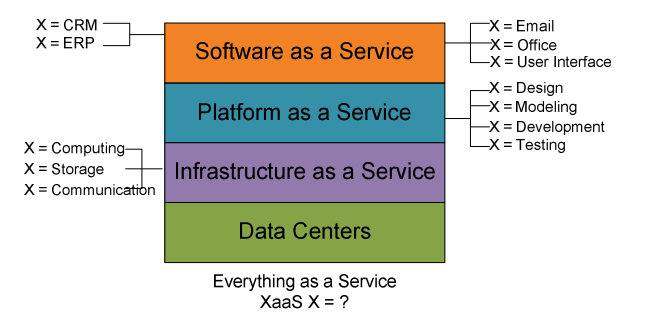
\includegraphics[width=.8\textwidth]{./images/high_level_cloud_view}
  \caption{Hierarchical View of Cloud Computing.}
  \label{fig:high_level_cloud_view}
\end{figure}\\
Data Centers allocates all the hardware that supports the cloud, they consist of thousands of physical machines that provides redundancy and ensure reliability in case of site failures. By using the IaaS pattern, Cloud Computing is able to virtualize
resources as computing power, storage and network connectivity of the data centers. These computational resources are provisioned on demand in a form of Virtual Machines (VM's) deployed in a cloud provider data-center \cite{sotomayor2009virtual}.
Cloud also assists application design, development, application hosting and testing by providing a development platform in order to assist the execution of these tasks, this development as a service pattern is know as PaaS. Another pattern supported by Cloud Computing
is SaaS. This pattern allows that a single piece of software is transferred to millions of users through a browser \cite{zhang2010cloud}. This pattern is beneficial by both users and developers, the developers only needs to maintain a single program while the users can
save costs in servers and software.\\

In a global analysis Cloud computing offers several benefits such as high-availability, high-scalability, flexibility, on-demand service provisioning and massive reduction of costs. By converging IoT applications and Cloud computing, IoT applications are able to take advantage
of all these benefits.
% -----------------------------------------
% CLOUD ORCHESTRATION
% -----------------------------------------
\subsubsection{Cloud Orchestration}
\label{subs:cloud_orchestration}
Due the heterogeneity of IoT applications infrastructure service management tasks such as deployment, driver installation and gateway configuration are still handled manually in a particular way for each case.
In order to reduce the complexity of this tasks, Cloud Orchestration tools can be used to automate these management tasks. The process of orchestration woven the software components of the application
in a one piece that can be managed more effectively, in order to ensure a smooth and fast service delivery. Cloud Orchestration helps to take advantage of the full benefits of Cloud computing by providing features that can include:
% Orchestration Features
\begin{itemize}
  \item Simplify, automate and optimize service deployment by integrating cloud capabilities across heterogeneous environments.
  \item Automated high-scale provisioning and de-provisioning of resources with policy-based tools.
  \item Real-time monitoring of physical and virtual Cloud resources.
  \item Selection of Cloud services such as storage and hosting, through a self-service portal.
  \item Real-time monitoring of usage and accounting chargeback capabilities to track and optimize system usage.
\end{itemize}
In addition, orchestration allows to reduce significantly the costs related with labor and resources, since that manual intervention and management of varied IT services and resources are not needed. Actually several tools to
performing Cloud Orchestration are available in the market such as IBM Cloud Orchestrator\footnote{http://www.ibm.com/software/products/en/ibm-cloud-orchestrator}, HP Operations Orchestration\footnote{http://www8.hp.com/us/en/software-solutions/operations-orchestration-it-process-automation}
and GigasSpaces Cloudify\footnote{http://www.gigaspaces.com/cloudify-cloud-orchestration/overview} and some open-source tools like Ubuntu Juju\footnote{http://www.juju.ubuntu.com} and OpenTOSCA\footnote{http://www.iaas.uni-stuttgart.de/OpenTOSCA/indexE.php}.\\

The remainder of this document is organized as the follows. In Section \ref{sec:objectives} we describe the problem to be solved as well the main objectives of this work. Section \ref{sec:related_work} presents the related work in the research area. Then in Section
\ref{sec:solution_architecture} we present a brief description of the state of art solution and propose the architecture for our solution. In Section \ref{sec:evaluation} the evaluation methodology is described. In the Section \ref{sec:conclusion} we presents the conclusion and finally
in the appendix we present the schedule for the future work.
